\chapter{Entwicklung des Prototpys für IntelliJ}
\label{cha:EntwicklungIntelliJ}

\section{Design}
\label{sec:EntwicklungIntelliJ_Design}

Wie schon in Kapitel \ref{cha:EntwicklungVsCode}, setzt sich das 
beschriebene Plugin in IntelliJ durch die Komponenten zusammen,
die in Abbildung \ref{fig:diagram_IntelliJDesign-Simplified} abgebildet sind.

\begin{figure}
    \centering
    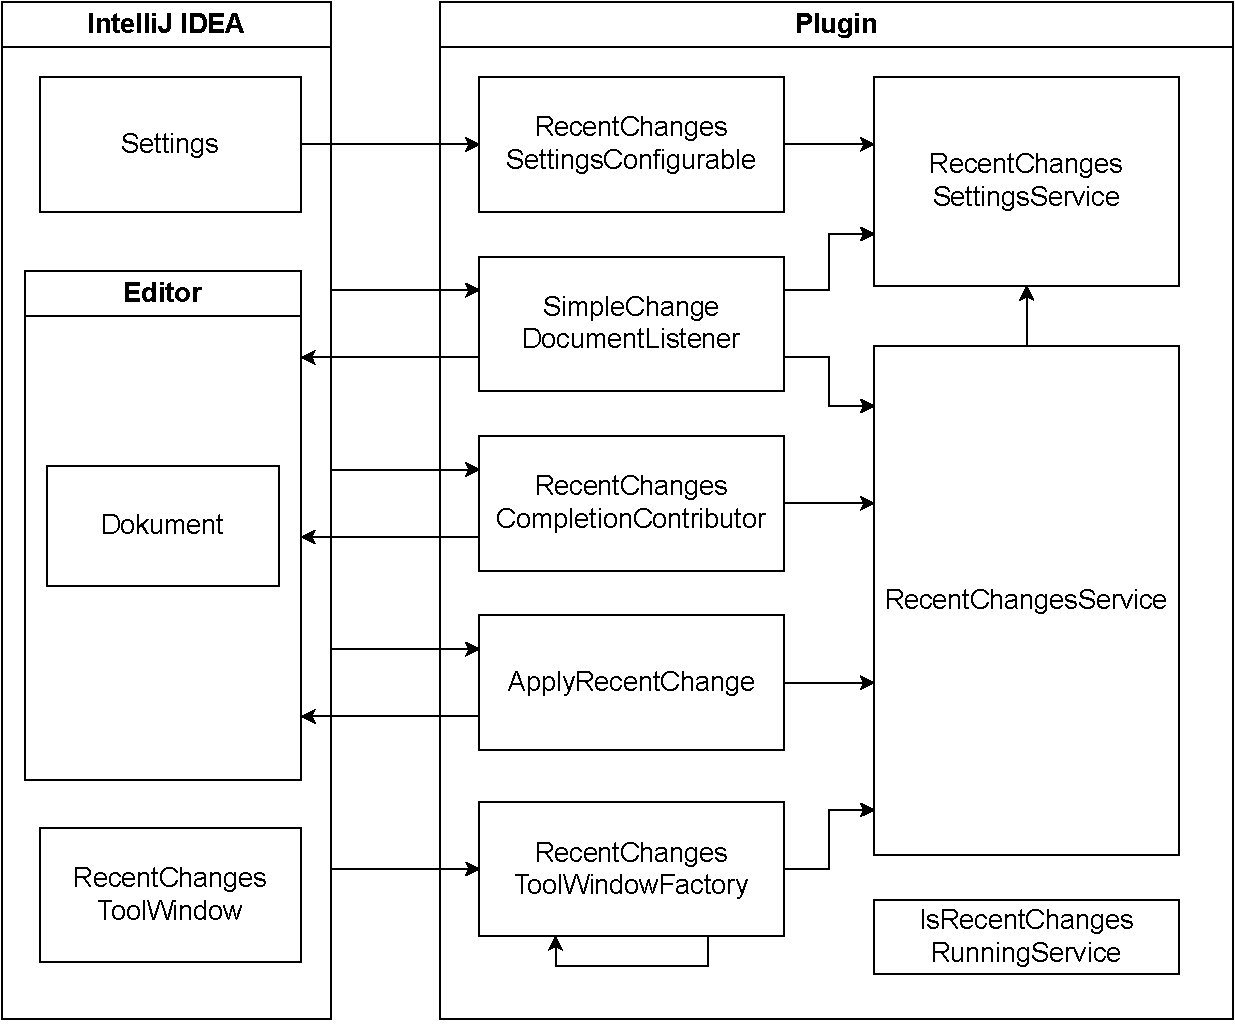
\includegraphics[width=.95\textwidth]{diagram_IntelliJDesign-Simplified}
    \caption{Stark vereinfachte Übersicht über das Design des Plugins in IntelliJ.}
    \label{fig:diagram_IntelliJDesign-Simplified}
\end{figure}

Da die beiden Plugins im Aufbau sehr ähnlich sind, sind auch die Aufgaben der
Einzelnen Komponenten beinahe deckungsgleich. Die Unterschiede liegen eher in
den Details.

Der \emph{SimpleChangeDocumentListener} übernimmt hier die Aufgabe,
des Beobachten des geöffneten Dokuments auf Veränderungen. Wird
eine Änderung festgestellt, so wird diese an den \emph{RecentChangesService}
zur Speicherung übergeben. Im Gegensatz zum \emph{RecentChangeStorage}
ist dieser allerdings als expliziter Service deklariert, der von IntelliJ
selbst verwaltet wird.

Die Komponenten für Einstellungen teilen sich auf 
\emph{RecentChangesSettingsConfigurable} und \emph{RecentChangesSettingsService}
auf. Die Klasse \emph{RecentChangesSettingsConfigurable} kümmert sich dabei
um die Darstellung und die Interaktivität der Einstellungen in der Benutzerschnittstelle.
Die Klasse \emph{RecentChangesSettingsService} wird wieder als Service 
angeboten und kümmert sich um das Speichern, Auslesen und Persistieren
der Einstellungen.

Die Codevervollständigung wird im IntelliJ Plugin durch den
\emph{RecentChangesCompletionContributor} durchgeführt. Dieser
sucht im \emph{RecentChangesService} nach Änderungen, die auf
das ausgewählte Wort passen und gibt diese als Vorschläge zurück.

Für das Einsetzen der Änderungen im Editor wird die Klasse
\emph{ApplyRecentChange} verwendet, die als Action registriert ist.
Bei der Action ist wie bereits im VS Code Plugin eine Tastenkombination
zum schnelleren Aufrufen hinterlegt.
Sollte keine passende Änderung gefunden werden, so wird direkt im
Editor ein Warnhinweis mit einer entsprechenden Meldung angezeigt.

Die Klasse \emph{RecentChangesToolWindowFactory} ist für die Darstellung
einer UI-Komponente zuständig, die dem TreeView aus dem VS Code Plugin
ähnelt. Sie ließt dafür den Zustand des \emph{RecentChangesService} aus
und baut eine entsprechende Baumstruktur auf. Um die Ansicht auch zum richtigen
Zeitpunkt aktualsieren zu können, wird der Service mithilfe eines
Observer-Patterns \cite{2005Dp:e} beobachtet.

Die Komponente \emph{IsRecentChangesRunningService} existiert für den Fall,
das zwei Instanzen von IntelliJ gleichzeitig auf einem Gerät gestartet werden.
Beim Start der Anwendung, müssen nämlich einige Initialisierungen vorgenommen
werden, die nur einmalig durchgeführt werden dürfen. Gegen den
\emph{IsRecentChangesRunningService} kann auf diese Weise geprüft werden, ob
die Initialisierung noch nötig ist, oder bereits gemacht wurde.


\section{Implementierung}
\label{sec:EntwicklungIntelliJ_Implementierung}

\subsection{Aufsetzen des Projektes}

% //TODO source

Das Erstellen eines neuen Plugin-Projektes kann in IntelliJ über den 
\enquote{New Project Wizard} erledigt werden. Dafür muss einfach
im Programm IntelliJ IDEA das Menü \emph{File -> New -> Project...}
gewählt werden. Hier gibt auf der linken Seite des Fensters eine 
Liste mit Projekt-Vorlagen, in welcher sich auch der Eintrag 
\emph{IDE Plugin} befindet. Für diesen Projekttyp kann dann unter anderem
ein Name für das Projekt gewählt werden. Dieser Name wird initial auch als
Name des Plugins verwendet.

Die durch IntelliJ generierte Ordnerstruktur kann (ausschnittsweise) in 
Abbildung \ref{fig:intellij_generated_structure} betrachtet werden.
Relevant ist hier vor allem die Datei \emph{plugin.xml}, die das 
enstprechend vorbereitete Plugin Manifest beinhaltet. Der Ordner
\emph{kotlin} ist als Verzeichnis für den Plugin-Code vorgesehen.
Er kann allerdings je nach Präferenz auch durch einen Ordner \emph{java}
ersetzt werden. Ein Ordner für Tests wird nicht automatisch generiert
und muss manuell hinzugefügt werden.

\begin{figure}
    \centering
    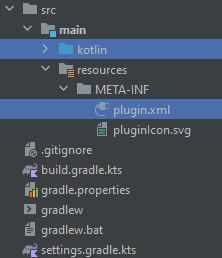
\includegraphics[width=.35\textwidth]{intellij_generated_structure}
    \caption{Ausschnitt der durch \emph{IntelliJ IDEA} generierten Ordnerstruktur.}
    \label{fig:intellij_generated_structure}
\end{figure}   

\subsection{Entwicklung}

\subsubsection{RecentChangesService}

Die Klasse \emph{RecentChangesService} (dargestellt in
Abbildung \ref{fig:diagram_IntelliJDesign-Detail_Service}) 
wird in der Form eines
Services auf Applikationsebene implementiert. Dies wird 
über das Attribut \emph{@Service(Service.Level.APP)} festgelegt. 
Auf diese Weise kann eine Instanz der Klasse in der gesamten Anwendung
bereitgestellt werden. Die statische Methode \emph{getInstance}
abstrahiert dabei die Aufrufe der IntelliJ API, die nötig sind um eine
Referenz auf diese Instanz zu erhalten. Genau wie im VS Code Plugin,
werden die Änderungen in einer \emph{EvictingQueue} von 
\emph{SimpleDiff}-Objekten gespeichert. Allerdings muss diese
Warteschlange hier nicht selbst implementiert werden, da es in
der Bibliothek \emph{Guava} von Google bereits eine etablierte 
Implementierung gibt. % //TODO source
Diese Bibliothek kann einfach
in der Datei \emph{build.gradle.kts} eingebunden werden.
Die verschiedenen Methoden der Klasse \emph{RecentChangesService} erlauben
das Einfügen, sowie das Auslesen, von \emph{SimpleDiff}-Objekten aus
der darunterliegenden Datenstruktur. Über die Methoden \emph{addChangeListener},
\emph{removeChangeListener} und \emph{notifyListeners} wird ein Observer-Pattern
abgebildet. Observer, welche die eigens erstellte Schnittstelle 
\emph{RecentDiffsChangedListener} implementieren, können sich also
beim \emph{RecentChangesService} anmelden. Sie werden dann bei Änderungen 
an den Daten über die Methode \emph{notifyChanged} notifiziert.
Da es sich bei der Klasse \emph{RecentChangesService} aufgrund der Implementierung
als IntelliJ Service um eine Singleton-Klasse % //TODO source
handelt, wird zusätzlich eine Methode \emph{reset} benötigt, um beim Testen
die Unabhängigkeit der verschiedenen Unit-Tests zu erhalten. Da für
die einzelnen Testfälle keine neuen Instanzen erzeugt werden können, muss
die Klasse also vor jedem Test zurückgesetzt werden.

\begin{figure}
    \centering
    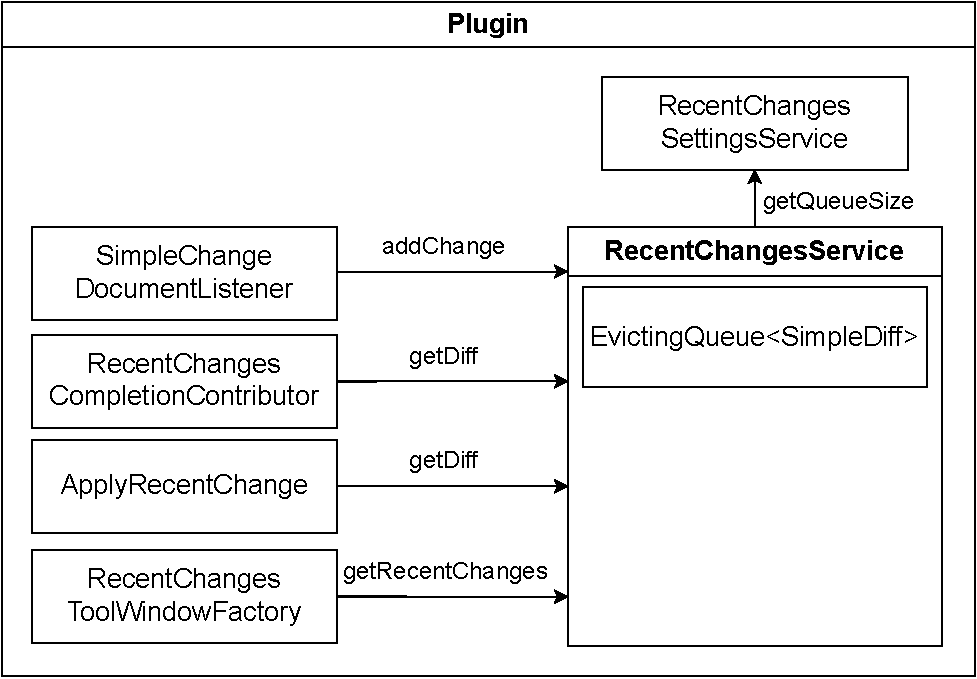
\includegraphics[width=.95\textwidth]{diagram_IntelliJDesign-Detail_Service}
    \caption{Detaillierte Darstellung des \emph{RecentChangesService}.}
    \label{fig:diagram_IntelliJDesign-Detail_Service}
\end{figure}

\subsubsection{SimpleChangeDocumentListener}

Der detaillierte Aufbau der Komponente \emph{SimpleChangeDocumentListener}
kann in Abbildung \ref{fig:diagram_IntelliJDesign-Detail_Listener} betrachtet werden.
Eine Instanz der Klasse wird beim ersten Start von IntelliJ als so registriert, 
dass er über die Änderungen in \emph{allen} geöffneten Dokumenten informiert wird. 
Hierfür muss die Schnittstelle \emph{DocumentListener} implementiert werden.
Diese definiert unter anderem die Methodensignaturen \emph{beforeDocumentChange}
und \emph{documentChanged}. Durch das Zusammenspiel dieser beiden Methoden
wird der gewünschte Debounce-Effekt erzeugt. Zu Beginn einer Änderung
wird in der Methode \emph{beforeDocumentChange} der aktuelle Text aus der 
unveränderten Datei ausgelesen. In der Methode \emph{documentChanged} wird
dann ein Timer gestartet (oder neu gestartet, falls er bereits laufen sollte).
Erst nach Ablauf des Timers (ohne einer weiteren Eingabe) wird
eine Änderung als abgeschlossen erkannt. Sobald dies geschieht, wird 
der Algorithmus \emph{diff-match-patch} verwendet um die Änderung zu analysieren.
Wird daraufhin festgestellt, dass es sich um eine einfache Änderung handelt,
so wird diese in den Speicher des \emph{RecentChangesService} eingefügt.
Zu beachten ist in dieser Klasse weiters die private Methode 
\emph{getOriginalTextFromDocument}. Dieser komplexe Aufruf
ist in IntelliJ notwendig, um den reinen Text des veränderten Dokuments
zu erhalten. Die Klasse \emph{Document} hätte zwar eigentlich
eine Methode \emph{getText}, dieser Text befindet sich aber möglicherweise
in einem Zwischenzustand, in dem IntelliJ spezielle Zeichenketten 
einsetzt, um die Anzeige der Codevervollständigung zu erleichtern.
% //TODO source IntelliJIdeaRulezzz https://intellij-support.jetbrains.com/hc/en-us/community/posts/206752355-The-dreaded-IntellijIdeaRulezzz-string
Um die originale Datei (und nicht eine modifizierte Kopie) zu erhalten
müssen also einige Umwege gegangen werden.

\begin{figure}
    \centering
    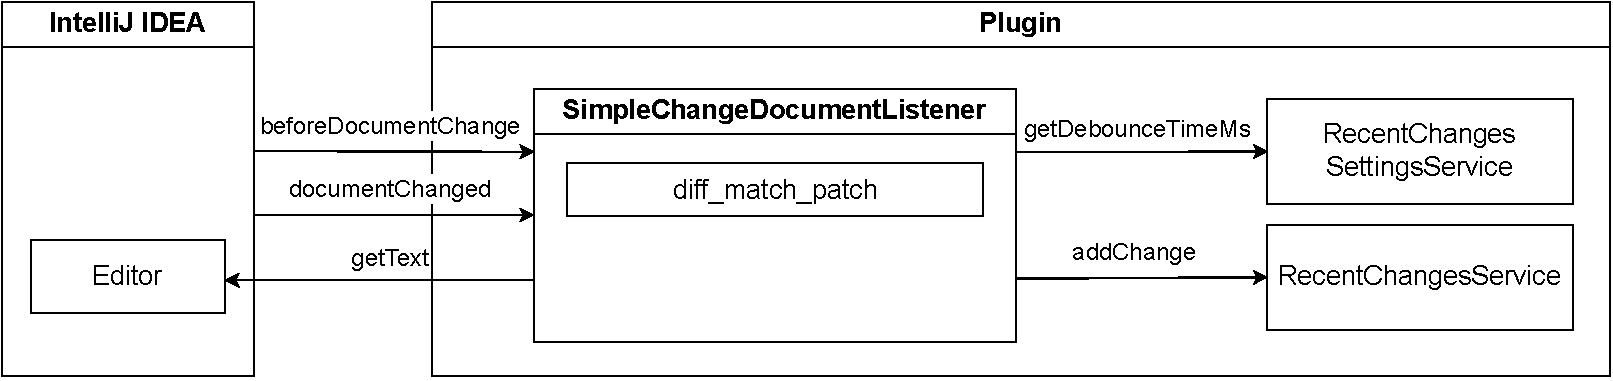
\includegraphics[width=.95\textwidth]{diagram_IntelliJDesign-Detail_Listener}
    \caption{Detaillierte Darstellung des \emph{SimpleChangeDocumentListener}.}
    \label{fig:diagram_IntelliJDesign-Detail_Listener}
\end{figure}

\subsubsection{ApplyRecentChange}

Bei \emph{ApplyRecentChange} handelt es sich um eine von
\emph{AnAction} abgeleitete Klasse. In Abbildung
\ref{fig:diagram_IntelliJDesign-Detail_Action} sind die Interaktionen
der Klasse dargestellt. Die Methoden \emph{actionPerformed} und \emph{update}
werden von IntelliJ aufgerufen. In beiden Methoden muss zuerst
der Inhalt der Datei an der aktuellen Position gelesen werden, um 
herauszufinden, ob das Anwenden der Action momentan möglich ist.
Sollte das Anwenden nicht möglich sein, wird
in der Methode \emph{update} mithilfe des übergebenen
\emph{AnActionEvent}-Objekt die Sichtbarkeit der Action (in den
registrierten Menüs des User Interface) entsprechend gesetzt.
In der Methode \emph{actionPerformed} wird in einem solchen Fall
eine Fehlermeldung mithilfe des IntelliJ Services \emph{HintManager}
angezeigt. Sollte ein ersetzen möglich sein,
so wird mittels der statischen Methode 
\emph{WriteCommandAction.runWriteCommandAction} ein Schreibbefehl
abgesetzt, in welchem der zu ersetzende Inhalt des Dokuments 
ausgetauscht wird. Dies ist nur über einen solchen Schreibbefehl möglich,
da ansonsten Synchronisationsprobleme auftreten könnten.
% //TODO source https://plugins.jetbrains.com/docs/intellij/working-with-text.html#safely-replacing-selected-text-in-the-document
% //TODO source https://plugins.jetbrains.com/docs/intellij/general-threading-rules.html#read-access
Im Manifest des Plugins wird die Action mit der 
Tastenkombination \emph{alt + R} registriert, um
auch Aufrufbar zu sein.

\begin{figure}
    \centering
    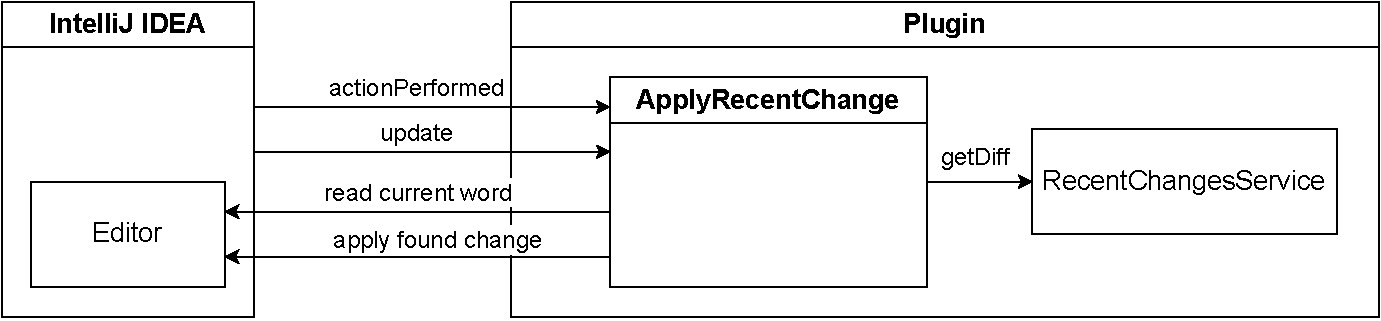
\includegraphics[width=.95\textwidth]{diagram_IntelliJDesign-Detail_Action}
    \caption{Detaillierte Darstellung der Action \emph{ApplyRecentChange}.}
    \label{fig:diagram_IntelliJDesign-Detail_Action}
\end{figure}

\subsubsection{RecentChangesCompletionContributor}

Die Klasse \emph{RecentChangesCompletionContributor}, die in Abbildung
\ref{fig:diagram_IntelliJDesign-Detail_Contributor} dargestellt wird,
leitet von \emph{CompletionContributor} ab. Im Konstruktor muss
die Methode \emph{extend} aufgerufen werden, der eine Instanz 
des eigentlichen \emph{CompletionProvider} übergeben wird.
Dieser \emph{CompletionProvider} überschreibt wiederum die 
Methode \emph{addCompletions}, welche die eigentliche Arbeit erledigt.
Genau wie bei der Action \emph{ApplyRecentChange}, wird der
Inhalt der Datei an der aktuellen Position ausgelesen. Das gefundene
Wort wird im \emph{RecentChangesService} nachgeschlagen.
Falls eine passende Änderung gefunden wird, wird diese über den 
Parameter \emph{resultSet} zu den Vorschlägen für die Codevervollständigung
hinzugefügt.
Im Manifest wird der Contributor für die Sprache \emph{any} registriert,
um Sprachunabhängig zu funktionieren.

\begin{figure}
    \centering
    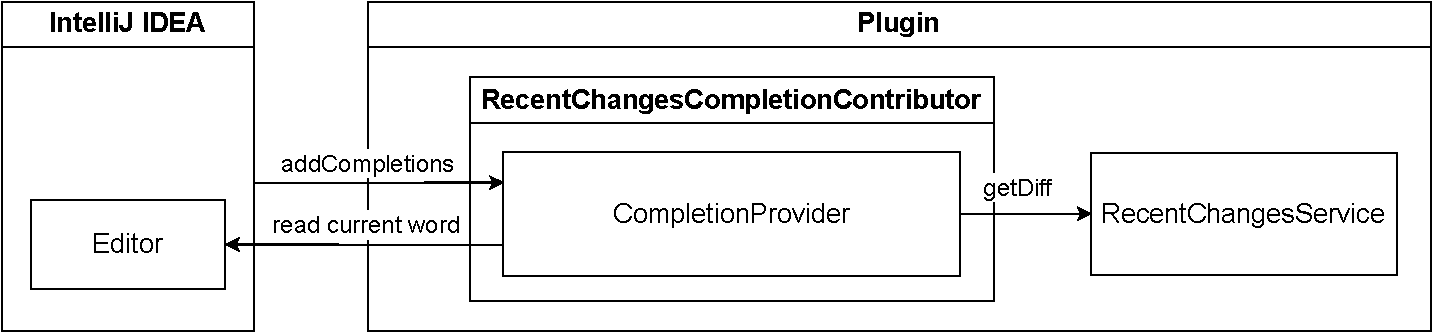
\includegraphics[width=.95\textwidth]{diagram_IntelliJDesign-Detail_Contributor}
    \caption{Detaillierte Darstellung des \emph{RecentChangesCompletionContributor}.}
    \label{fig:diagram_IntelliJDesign-Detail_Contributor}
\end{figure}

\subsubsection{RecentChangesToolWindowFactory}

Die Klasse \emph{RecentChangesToolWindowFactory} ist in Abbildung
\ref{fig:diagram_IntelliJDesign-Detail_ToolWindow} dargestellt.
Sie implementiert die Schnittstelle \emph{ToolWindowFactory} 
und überschreibt die Methode \emph{createToolWindowContent}. Zur besseren 
Abgrenzung der Aufgaben, wird in dieser zuerst eine neue Instanz
der Klasse \emph{RecentChangesToolWindowContent} erstellt.
Diese innere Klasse verwaltet den Inhalt und das Aussehen des Fensters.
Sie lädt die nötigen Daten aus dem \emph{RecentChangesService} und
meldet sich bei dem Service auch als Listener an, um gegebenenfalls den
Inhalt zu aktualisieren. Die Darstellung des Fensterinhalts
geschieht über ein \emph{JPanel} aus Java Swing und einem \emph{Tree}
aus der UI-Bibliothek von IntelliJ. Dieser Inhalt wird
durch die Methode \emph{getContentPanel} von außen zugänglich gemacht.
Zum Schluss setzt die Methode \emph{createToolWindowContent} 
den eigentlichen Inhalt des Fensters durch den Aufruf von
\emph{toolWindow.getContentManager().addContent} auf dem übergebenen
Parameter.
Im Manifest wird \emph{RecentChangesToolWindowFactory} als Factory-Klasse
für ein ToolWindow namens \emph{Recent Changes} registriert.

\begin{figure}
    \centering
    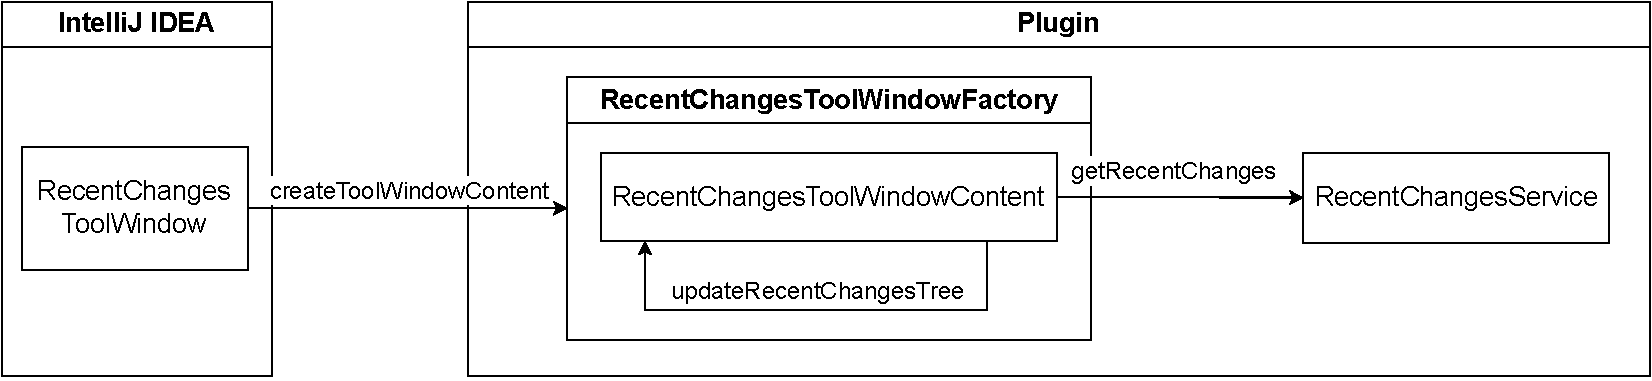
\includegraphics[width=.95\textwidth]{diagram_IntelliJDesign-Detail_ToolWindow}
    \caption{Detaillierte Darstellung der \emph{RecentChangesToolWindowFactory}.}
    \label{fig:diagram_IntelliJDesign-Detail_ToolWindow}
\end{figure}

\subsubsection{Einstellungen}

Die für die Einstellungen nötigen Klassen sind in Abbildung
\ref{fig:diagram_IntelliJDesign-Detail_Settings} zu sehen.
\emph{RecentChangesSettingsConfigurable} ist die Hauptschnittstelle 
zu IntelliJ, die auch im Manifest entsprechend registriert ist. 
Sie implementiert das Interface \emph{Configurable}
und bietet verschiedene Methoden an, die für die Darstellung
und Interaktivität in der Benutzerschnittstelle nötig sind.
Durch die Methode \emph{apply} sollen die aktuell gewählten Einstellungen
persistiert werden. Durch die Methode \emph{reset} sollen die 
zuvor gespeicherten Einstellungen wieder angezeigt werden.
Durch die Methode \emph{isModified} wird überprüft, ob die angezeigten
Einstellungen von den persistierten Einstellungen abweichen. 
Ist dies nicht der Fall, wird der Knopf zum Speichern der Einstellungen
automatisch ausgegraut. Die Methode \emph{createComponent} stellt
den Inhalt der Einstellungsseite in Form eines \emph{JComponent} bereit.
Um gute Aufgabenteilung zu ermöglichen, ist diese Darstellung an die 
Klasse \emph{RecentChangesSettingsComponent} ausgelagert. Sie beinhaltet
Felder zum Eingeben der Warteschlangengröße und der Debouncezeit.
Über Getter- und Setter-Methoden können diese Werte von 
\emph{RecentChangesSettingsConfigurable} beliebig verwaltet werden.
Um das Eingeben von ungültigen Werten zu vermeiden, werden zusätzlich
Filter auf die Eingabefelder angewandt.
Der \emph{RecentChangesSettingsService} ist die Komponente die für das 
Persistieren der Einstellungen verantwortlich ist. Hierfür
wird die Schnittstelle \emph{PersistentStateComponent} implementiert
und das Attribut \emph{@State} angegeben. Auf diese Weise ruft
IntelliJ zu den passenden Zeitpunkten automatisch die Methoden
\emph{getState} und \emph{loadState} auf und serialisiert den Zustand
in einer \emph{.xml}-Datei.
Zusätzlich ist die Klasse im Manifest als Service registriert, und bietet
passende Methoden zum Auslesen und Setzen, sowie ein Observer-Pattern
zum Beobachten der Einstellungen, an.

\begin{figure}
    \centering
    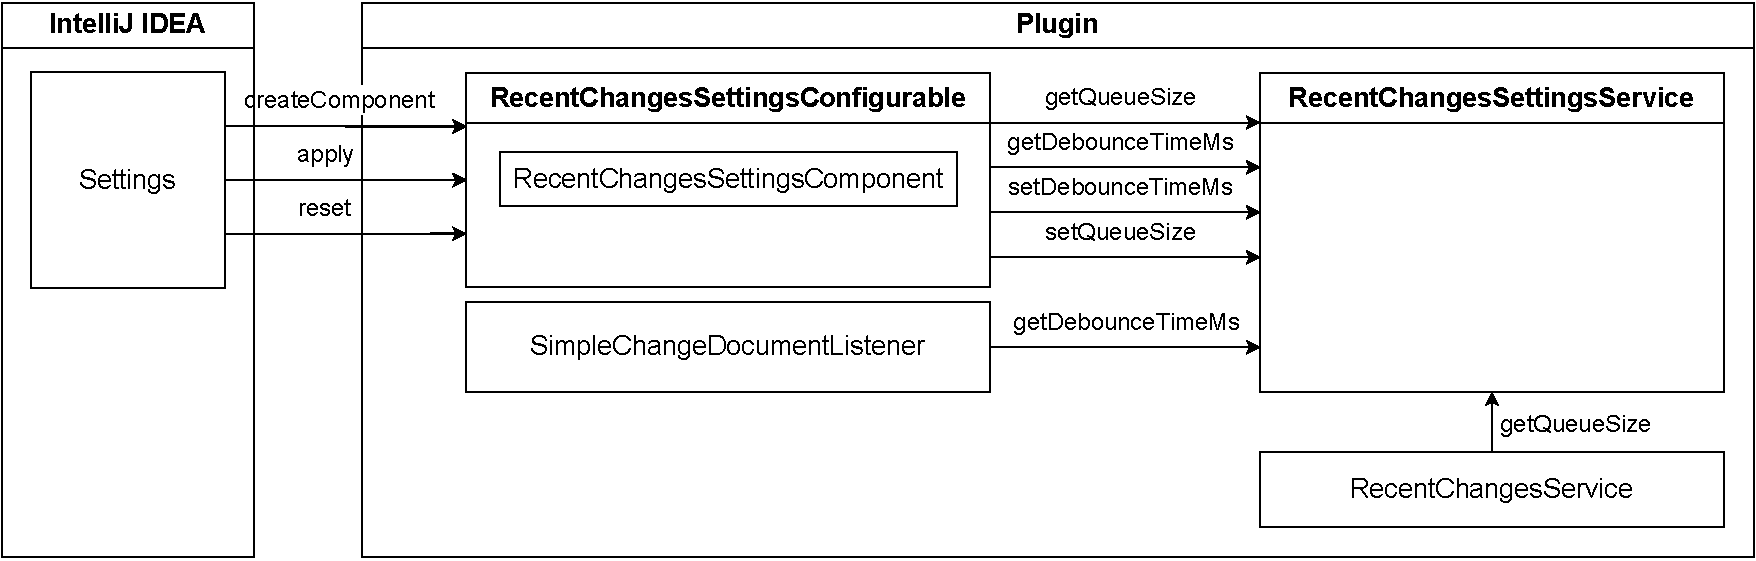
\includegraphics[width=.95\textwidth]{diagram_IntelliJDesign-Detail_Settings}
    \caption{Detaillierte Darstellung der \emph{Settings} Komponenten.}
    \label{fig:diagram_IntelliJDesign-Detail_Settings}
\end{figure}

\section{Tests}
\label{sec:EntwicklungIntelliJ_Tests}

\section{Publishing}
\label{sec:EntwicklungIntelliJ_Publishing}

\section{CI/CD}
\label{sec:EntwicklungIntelliJ_CICD}